\documentclass[10pt]{beamer}
\usepackage{uglixbeamer,animate}

\subtitle{Chapitre 01}
\title{Variables et affectation}
\author{NSI1}
\begin{document}

\maketitle
\begin{frame}{Qu'est-ce qu'une variable ?}\pause
\begin{center}
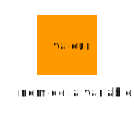
\includegraphics[width=7cm]{img/variable}
\end{center}
\end{frame}

\begin{frame}{Différence avec les maths}\pause
\begin{center}
\includegraphics[width=7cm]{img/different}
\end{center}
\end{frame}

\begin{frame}{En mathématiques}\pause
\huge
\begin{enumerate}[\textbullet]
	\item  $2+2=4$\pause
    \item  $\mathcal{P}=2\times(l+L)$\pause
    \item  Pour tout $x\in\R$, $f(x)=x^2+1$\pause
    \item  $2x+1=3x-2$\pause
    \item $A=2\times (\frac{3}{7}-\frac{8}{3})$
\end{enumerate}
\end{frame}

\begin{frame}[fragile]{En \textsc{Python}}\pause
\begin{minted}[fontsize=\huge]{python}
a = 1
\end{minted}
\pause

\begin{minted}[fontsize=\huge]{python}
x = 0
x = x + 1
\end{minted}
\pause

\begin{minted}[fontsize=\huge]{python}
a = 2
b = 3
c = (7 * b - 2 ) / a
\end{minted}

\end{frame}

\begin{frame}{Conclusion}
En mathématiques, le signe $=$ a de multiples interprétations.\\\pause

En \textsc{Python} il n'en a qu'une : l'affectation.\pause

\begin{center}
\includegraphics[width=7cm]{img/affectation}
\end{center}
\end{frame}

\end{document}
